\Chapter{Az elkészült függvénykönyvtár bemutatása}

% TODO: Példák kellenének, hogy egy-egy probléma megoldására hogyan használható az elkészített szoftver.
\Section{Útvonalkereső algoritmus}

A programrészek készítésekor próbáltam arra törekedni, hogy minél jobban személyre szabhatóbbak legyenek az egységek. Az A* algoritmus integrálása ezáltal úgy történhet, hogy mi magunk definiálhatunk egy környezetet, amiben a keresés fog történni. Ez ugyan időt vesz igénybe, viszont olyan pályát tudunk készíteni, amilyet mi szeretnénk. Továbbfejlesztési lehetőség lenne, hogy ne csak téglalap alakú objektumokat tudjunk meghatározni, hanem egyéb más alakzatokat is, így viszont további függények kellenének a pontok akadályba ütközésének vizsgálatára.

\subsection{A* felhasználási módja}

A programban az algoritmus működéséhez szükséges számításokat osztályba szerveztem, ahol függvények vannak definiálva erre a célra. Név szerint AStarPathFinder()-ként szerepel. Magát az osztályt inicializálni kell az akadályokkal, ami majd a környezetet adja, hasonlóan, ahogy a példában is szerepel:

\begin{figure}[h!]
\centering
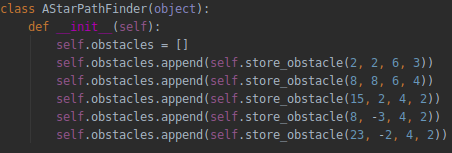
\includegraphics[scale=0.75]{images/store_obstacles.png}
\caption{Akadályok tárolása}
\label{fig:store_obstacles}
\end{figure}

Külön függvény fogja összegyűjteni az akadályok pontjait, nekünk elég csak a kezdőpontot, valamint a szélességet és a magasságot megadni. Ezt az osztályt érdemes külön modulba kiszervezni, valamint az algoritmust egy másik metódus valósítja meg. Ezért fontos, hogy az osztály metódusai elérhetőek legyenek a keresést megvalósító függvény számára. Ehhez példányosítani kell az osztályt, és a függvény harmadik paramétere lenne ez a példány, amikor meghívjuk. A kereső algoritmus így fogja felismerni az osztályon belül definiált metódusokat. Visszatérési értékként megkapjuk az útvonal koordinátáit, valamint a költséget. Eldönthetjük mire lesz szükségünk ezek közül és ez alapján valamilyen formában ezt megjeleníteni.

\Section{A jármű mozgása}

A jármű mozgását szimuláló programrész pedig megoldást ad a a mozgás során fellépő problémákra. Végeredményként animációkat tudunk készíteni vele és tudjuk elemezni, amit leprogramoztunk. 

\subsection{A mozgatás felhasználási módja}
Egy python fájlban található minden, ami szükséges a futtatáshoz. Lényegében 3 függvény és egy $ main $ segítségével működik az egész, valamint globális változókkal. Ezeket lehet fix értékekkel helyettesíteni, a tesztelés miatt volt szükség a kiszervezésükre, hogy több esetet tudjak generálni a parkolós mozgásra. Lehetőség van még a jármű méretének beállítására is:

\begin{figure}[h!]
\centering
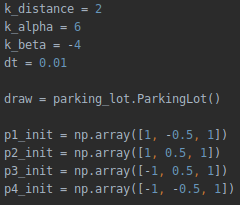
\includegraphics[scale=0.75]{images/init_for_vehicle_moving.png}
\caption{Inicializálás}
\label{fig:init_for_vehicle_moving}
\end{figure}

A fájlon belül a $ moving\_vehicle $ függvény hívja meg a kirajzoló metódust, ami pedig a rotációs mátrixot, így ezeket célszerű együtt tárolni. A kirajzoló függvényt lehet helyettesíteni a felhasználási célnak megfelelő egyéb függvényekkel. Viszont ehhez a jármű pontjait meghatározó mátrix szorzást is át kell helyeznünk. Ennek pedig minden lépésnél le kell futnia, így kaphatjuk vissza mindig a forgatott járművet.

\begin{figure}[h!]
\centering
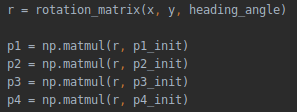
\includegraphics[scale=0.75]{images/rotation.png}
\caption{A jármű négy pontja}
\label{fig:rotation}
\end{figure}

